\documentclass[11pt]{article}

\usepackage[margin=1.15in]{geometry}
\usepackage{amsmath, amssymb}
\usepackage{booktabs}
\usepackage{graphicx}
\usepackage{array}
\usepackage{longtable}
\usepackage[hidelinks]{hyperref}
\usepackage{caption}
\usepackage{enumitem}
\usepackage{xcolor}
\usepackage{listings}
\usepackage{siunitx}
\usepackage{microtype}
\sisetup{detect-all, group-separator={,}}

\captionsetup{font=small, labelfont=bf}
\setlist{itemsep=2pt, topsep=4pt}

\lstset{
  basicstyle=\ttfamily\footnotesize,
  breaklines=true,
  frame=single,
  framesep=4pt,
  rulecolor=\color{gray!50},
  backgroundcolor=\color{gray!5},
  columns=fullflexible,
}

\newcommand{\code}[1]{\texttt{\small #1}}

\title{\bfseries Physics-Informed Accelerated MRI Reconstruction\\
with SwinUNet: Auditing, Correcting, and Extending\\
a Transformer Reconstruction Pipeline}

\author{Matthew Park}
\date{July 2026}

\begin{document}
\maketitle

\begin{abstract}
\noindent
Magnetic Resonance Imaging provides detailed anatomical information without
ionising radiation, but its long acquisition times limit throughput and patient
comfort. Accelerated MRI addresses this by undersampling $k$-space and
reconstructing the missing information computationally. In earlier work I
proposed a hybrid U-Net/Swin Transformer architecture for this task and reported
that the SwinUNet variant reached \SI{33.10}{\decibel} PSNR on the fastMRI
single-coil knee benchmark, above a U-Net baseline at
\SI{28.03}{\decibel}.

This paper reports a systematic audit of the released implementation and a
substantially revised system. The audit found that the released code could not
execute: the SwinUNet could not be \emph{constructed} at its own documented
configuration, because window partitioning assumed feature-map resolutions
divisible by the window size and the third encoder stage is $20\times20$ with a
window size of $8$. Two further defects made every inference and evaluation
entry point raise on invocation. A second class of defects ran silently but
invalidated measurements: exponential-moving-average weights were never loaded,
the data-consistency module was never given data and was therefore a complete
no-op, the equispaced sampling mask acquired \SI{19.3}{\percent} more
$k$-space lines than its nominal acceleration, and PSNR was averaged over
mini-batches before the logarithm, which makes the metric depend on batch size.

I rebuild the system around the physics of the acquisition. Reconstruction is
performed on complex-valued data through an unrolled cascade in which every
learned refinement is followed by a data-consistency projection that restores
the measured Fourier coefficients exactly, verified here to
$8.3\times10^{-7}$. Metrics are computed per image against each target's own
dynamic range, and model comparisons report bootstrap confidence intervals and
Holm-corrected paired permutation tests rather than point estimates.

In a controlled ablation on synthetic phantom data with capacity-matched
controls, the data-consistency cascade improves reconstruction over an
equal-parameter single-pass network by a margin that is statistically
significant under a paired test. I do not restate the previously reported
fastMRI figures as validated results: they are not reproducible from the
released artifact, and the corrections to the sampling and metric definitions
mean that numbers produced under the old protocol are not comparable to numbers
produced under the new one. The revised system, its 217-test suite, and a
synthetic data generator that makes the full pipeline runnable without the
fastMRI download are released so that the benchmark numbers can be regenerated
under a protocol that is stated precisely and checked automatically.
\end{abstract}

\tableofcontents
\newpage

% =====================================================================
\section{Introduction}
% =====================================================================

Magnetic Resonance Imaging (MRI) is among the most valuable non-invasive
diagnostic modalities, offering exceptional soft-tissue contrast without
ionising radiation. Its principal limitation is time. A fully sampled
acquisition requires the scanner to traverse $k$-space line by line, which keeps
patients immobile for extended periods, reduces scanner throughput, invites
motion artefacts, and raises cost.

Accelerated MRI acquires only a fraction of $k$-space and recovers the remainder
computationally. Undersampling below the Nyquist rate makes the inverse problem
ill-posed: the naive zero-filled reconstruction exhibits coherent aliasing that
obscures precisely the fine structures---cartilage boundaries, meniscal tears,
cortical margins---that determine diagnostic value. Classical remedies include
parallel imaging (SENSE~\cite{pruessmann1999}, GRAPPA~\cite{griswold2002}) and
compressed sensing~\cite{lustig2007}. Deep learning has since become the
dominant approach, and the fastMRI benchmark~\cite{zbontar2018} has made
progress measurable.

\subsection{Motivation for this paper}

My earlier study compared a baseline U-Net, a U-Net with a Transformer at the
bottleneck (BT-UNet), and a SwinUNet, and reported that the SwinUNet reached
\SI{33.10}{\decibel} PSNR and \num{0.7274} SSIM, against \SI{28.03}{\decibel}
and \num{0.6935} for the U-Net. That gap is \SI{5.07}{\decibel}, though the
prose of that paper described it as ``approximately \SI{4}{\decibel}'' in three
places---the first and mildest of the inconsistencies this audit uncovered.

Preparing the work for release, I audited the implementation against its own
documentation. The audit did not find the small discrepancies one expects. It
found that the artifact could not run at all, and that several components which
appeared to be working were not.

The most consequential finding concerns the flagship model. With the documented
configuration---\SI{320}{px} input, patch size $4$, three encoder stages, window
size $8$---the stage resolutions are $80 \to 40 \to 20$. Window partitioning was
implemented as a reshape,
\begin{lstlisting}[language=Python]
x = x.view(B, H // ws, ws, W // ws, ws, C)
\end{lstlisting}
which silently requires $H$ and $W$ to be exact multiples of \code{ws}. At the
third stage $20 \bmod 8 \neq 0$, and because the shifted-window attention mask
was precomputed in \code{\_\_init\_\_}, the failure occurred at
\emph{construction}:
\begin{lstlisting}
RuntimeError: shape '[1, 2, 8, 2, 8, 1]' is invalid for input of size 400
\end{lstlisting}
No forward pass through the reported architecture was possible from the released
code. A separate misspelled module filename (\code{reproductibility.py}, imported
as \code{reproducibility}) made \code{import training} raise
\code{ModuleNotFoundError}, and two methods on the inference pipeline were
missing their \code{@classmethod} and \code{@staticmethod} decorators, so every
documented inference, benchmarking and export command raised immediately.

That a codebase in this state passed its own continuous-integration suite has a
mundane explanation that is worth recording: the workflow file was at
\code{.github/.workflows/ci.yml}. GitHub reads only
\code{.github/workflows/}, so CI had never run. The repository's
architecture-sanity command would not have caught it either---it wrapped each
forward pass in a bare \code{except}, printed \code{FAIL} into a formatted
table, and exited with status~0.

\subsection{Contributions}

\begin{enumerate}[leftmargin=*]
  \item \textbf{A reproducibility audit} of the released implementation,
        classifying 19 defects into those that prevent execution, those that
        run but silently disable a documented feature, and those that corrupt
        measurement. Each is characterised by mechanism and, where it affects
        reported numbers, quantified (Section~\ref{sec:audit}).
  \item \textbf{A corrected and generalised SwinUNet}. Feature maps are padded
        to the window size with padded tokens masked out of attention, so any
        resolution and any window size are valid; attention masks are built
        lazily and cached per resolution rather than baked in at construction.
        The architecture gains stochastic depth, truncated-normal
        initialisation, fused attention, and a zero-initialised residual head
        that makes the network the exact identity at step~0
        (Section~\ref{sec:swinunet}).
  \item \textbf{A physics-informed reconstruction pipeline}. Reconstruction
        operates on complex data through an unrolled cascade of learned
        refinements interleaved with data-consistency projections. I show the
        projection restores measured coefficients to $8.3\times10^{-7}$
        (Sections~\ref{sec:dc} and~\ref{sec:verification}).
  \item \textbf{A corrected simulation and evaluation protocol}: sampling masks
        that achieve their nominal acceleration, augmentation applied before
        undersampling so every training sample remains a realisable
        acquisition, per-image metrics against each target's own dynamic range,
        and comparisons reported with bootstrap confidence intervals and
        Holm-corrected paired permutation tests
        (Sections~\ref{sec:data} and~\ref{sec:evaluation}).
  \item \textbf{A controlled ablation} on synthetic phantom data with
        capacity-matched controls, isolating the contribution of complex-valued
        input and of the data-consistency cascade from that of parameter count
        (Section~\ref{sec:ablation}).
  \item \textbf{A verifiable artifact}: 217 automated tests including exactness
        assertions on the Fourier and data-consistency operators, schema
        validation that rejects invalid configurations before training starts,
        and a synthetic data generator that makes the entire pipeline runnable
        without the \SI{90}{\giga\byte} fastMRI download
        (Section~\ref{sec:artifact}).
\end{enumerate}

\subsection{What this paper does not claim}
\label{sec:not-claimed}

I do not report validated fastMRI benchmark results. The previously published
figures cannot be reproduced from the released code, and the corrections
described here---to the sampling mask, the metric definition, and the
augmentation ordering---change what those numbers measure, so old and new
results are not comparable. Producing new fastMRI numbers requires GPU-scale
training runs that are outside the scope of this paper. What is provided instead
is a system in which such numbers can be generated under a protocol that is
stated precisely, validated automatically, and reproducible from a recorded
commit. Section~\ref{sec:protocol} gives the exact commands.

% =====================================================================
\section{Related Work}
% =====================================================================

\subsection{Traditional reconstruction}

Parallel imaging exploits redundancy across receiver coils: SENSE unfolds
aliasing in image space using coil sensitivity maps~\cite{pruessmann1999}, while
GRAPPA interpolates missing $k$-space lines from autocalibration
data~\cite{griswold2002}. Compressed sensing instead exploits sparsity in a
transform domain and requires incoherent sampling~\cite{lustig2007}. These
methods are well understood and clinically deployed, but reconstruction is slow,
noise amplification grows with acceleration, and performance depends on
calibration data or on the sampling pattern's incoherence.

\subsection{Deep learning for MRI reconstruction}

Early learned approaches treated reconstruction as image-to-image
denoising~\cite{hyun2018, lee2018}. The more durable line of work embeds the
forward model in the network. Schlemper et al.~\cite{schlemper2018} introduced a
cascade of CNNs interleaved with data-consistency layers; Hammernik et
al.~\cite{hammernik2018} unrolled a variational optimisation into a trainable
network; Sriram et al.~\cite{sriram2020} extended this end to end with learned
coil sensitivities. The common principle---that a reconstruction network should
not be free to contradict the measurements---is the one this paper adopts, and
is what the original implementation attempted but did not achieve.

\subsection{Transformers for reconstruction}

Vision Transformers~\cite{dosovitskiy2020} showed that attention can replace
convolution for image tasks. Applying global attention at MRI resolutions is
prohibitive, since cost grows quadratically in token count. The Swin
Transformer~\cite{liu2021} resolves this with attention restricted to local
windows and a shifted partitioning between consecutive blocks, giving linear
cost in image area while still propagating information globally across depth.
Swin-UNet~\cite{cao2021} arranges this hierarchically for segmentation. For
reconstruction specifically, Lin and Heckel~\cite{lin2022} showed ViTs can match
U-Net performance, and Huang et al.~\cite{huang2022} combined deformable
attention with a U-Net.

The present work differs from my earlier study in emphasis. The earlier question
was which backbone reconstructs best. The question here is whether the
comparison was measured correctly at all, and---once the measurement is
trustworthy---how much of the achievable gain comes from the backbone versus
from respecting the acquisition physics.

% =====================================================================
\section{Reproducibility Audit}
\label{sec:audit}
% =====================================================================

This section documents the defects found in the released implementation. It is
included because the failure modes are not idiosyncratic: a metric that depends
on batch size, an undersampling mask that is denser than reported, and a
physics module that is silently inert are mistakes any reconstruction project
can make, and none of them announce themselves in a loss curve.

\subsection{Class 1: defects preventing execution}

\begin{table}[h]
\centering
\small
\begin{tabular}{@{}p{0.30\textwidth}p{0.62\textwidth}@{}}
\toprule
\textbf{Defect} & \textbf{Consequence} \\
\midrule
Window partition assumed divisible resolutions &
At the documented configuration the third encoder stage is $20\times20$ with
window size $8$. The precomputed shift mask made this a construction-time
\code{RuntimeError}, so the reported architecture never ran. \\[4pt]

\code{utils/reproductibility.py} misspelled &
\code{utils/\_\_init\_\_.py} imported \code{utils.reproducibility}, so
\code{import training} raised \code{ModuleNotFoundError}. Every training entry
point failed at import. \\[4pt]

\code{from\_checkpoint} and \code{\_build\_model} missing decorators &
Both were plain functions on the class. The documented call
\code{Pipeline.from\_checkpoint(path)} bound \code{path} to \code{cls}. All
inference, benchmarking and export commands raised on invocation. \\
\bottomrule
\end{tabular}
\caption{Defects that prevented any documented command from running.}
\end{table}

\subsection{Class 2: silent defects}

These executed without error while disabling a documented capability.

\begin{table}[h]
\centering
\small
\begin{tabular}{@{}p{0.30\textwidth}p{0.62\textwidth}@{}}
\toprule
\textbf{Defect} & \textbf{Consequence} \\
\midrule
\code{average\_parameters} lacked \code{@contextmanager} &
The method returned a bare generator, so \code{with ema.average\_parameters():}
executed an empty body. Validation reported raw training weights while
appearing to report EMA weights. \\[4pt]

EMA wrote \code{shadow}; loaders read \code{shadow\_params} &
The key never matched, so the fallback branch loaded raw weights. EMA was
computed throughout training and never used. \\[4pt]

Data-consistency wrapper guarded on \code{k\_measured is None} &
The trainer called \code{model(x)} with no $k$-space, so the guard skipped the
projection every time. The configuration flag
\code{data\_consistency.enabled} had no effect whatsoever. \\[4pt]

DC layer returned \code{x.abs()} &
Phase was discarded, so the operator could not be cascaded: the next transform
would treat a zero-phase image as the estimate. \\[4pt]

\code{sigmoid(lambda\_init)} &
A requested hard consistency of \num{1.0} became \num{0.7311}, admitting
\SI{27}{\percent} of network output into measured frequencies. \\[4pt]

Attention hooks read the forward output &
\code{WindowAttention} returns a tensor, not a tuple, and never stored weights.
Every attention figure was empty. \\[4pt]

CI at \code{.github/.workflows/} &
GitHub reads only \code{.github/workflows/}; CI had never executed. \\[4pt]

\code{test\_models} caught all exceptions, exited 0 &
The sanity check reported failure in its output table and success to the shell.
\\
\bottomrule
\end{tabular}
\caption{Defects that ran without error while disabling a documented feature.}
\end{table}

\subsection{Class 3: measurement defects}

These affect reported numbers and are quantified below.

\subsubsection{Sampling mask acceleration}

The equispaced mask was constructed by taking every $R$-th line and then adding
the fully sampled centre on top:
\begin{lstlisting}[language=Python]
mask[::acceleration] = 1.0
mask[pad : pad + num_low_freqs] = 1.0
\end{lstlisting}
This acquires $N/R + N\cdot\mathit{cf}$ lines rather than $N/R$. The nominal
acceleration is therefore not achieved. Table~\ref{tab:mask} gives measured
values over 200 draws at $N=368$.

\begin{table}[h]
\centering
\small
\begin{tabular}{@{}rrrrrr@{}}
\toprule
Nominal $R$ & centre fraction & original & error & corrected & error \\
\midrule
2  & 0.16 & 1.72  & $-14.0\%$ & 1.99  & $-0.3\%$ \\
4  & 0.08 & 3.23  & $-19.3\%$ & 4.00  & $+0.1\%$ \\
8  & 0.04 & 6.13  & $-23.3\%$ & 8.03  & $+0.4\%$ \\
16 & 0.02 & 12.27 & $-23.3\%$ & 16.01 & $+0.0\%$ \\
\bottomrule
\end{tabular}
\caption{Achieved acceleration of the equispaced mask. The original acquires
19--23\% more $k$-space than reported at clinically relevant factors, making the
reconstruction problem correspondingly easier than stated.}
\label{tab:mask}
\end{table}

\subsubsection{PSNR definition}

PSNR was computed as
\begin{equation}
\mathrm{PSNR}_{\text{batch}} = 10\log_{10}\!\left(\frac{1}{\frac{1}{B}\sum_b \mathrm{MSE}_b}\right),
\end{equation}
whereas the standard definition averages per-image values,
\begin{equation}
\mathrm{PSNR} = \frac{1}{B}\sum_b 10\log_{10}\!\left(\frac{\mathrm{max}_b^2}{\mathrm{MSE}_b}\right).
\end{equation}
Because $\log$ is concave, Jensen's inequality gives
$\mathrm{PSNR}_{\text{batch}} \le \mathrm{PSNR}$, with a gap that grows with the
variance of per-image MSE across the batch---and therefore with batch size.
Table~\ref{tab:psnr} reports the measured gap on heteroscedastic synthetic data.

\begin{table}[h]
\centering
\small
\begin{tabular}{@{}rrr@{}}
\toprule
Batch size & Gap (dB) & SD \\
\midrule
1  & 0.000 & 0.000 \\
2  & 1.111 & 1.334 \\
4  & 1.641 & 1.066 \\
6  & 1.674 & 0.874 \\
8  & 1.777 & 0.800 \\
16 & 1.922 & 0.621 \\
32 & 1.840 & 0.403 \\
\bottomrule
\end{tabular}
\caption{Per-image PSNR minus the batch-MSE formulation, over 200 trials. The
quantity being reported depends on a training hyperparameter. In the original
study the U-Net used batch size 8 and the SwinUNet batch size 6, a
configuration difference worth \SI{0.10}{\decibel} of pure measurement artefact
in the baseline's favour.}
\label{tab:psnr}
\end{table}

A second issue compounds this: the peak signal value was hard-coded to
\num{1.0}. Under per-slice normalisation the target maximum is not \num{1.0},
so the denominator was wrong by a per-sample factor. Both are corrected in
Section~\ref{sec:metrics}.

\paragraph{Evidence in the original figures.} The training curves published with
the prior study are reproduced in Figure~\ref{fig:prior-curves}, because they
document these defects directly rather than merely being consistent with them.

Three observations. First, the U-Net's SSIM panel oscillates between
\num{0.66} and \num{0.74} from epoch to epoch for sixty epochs and never
converges, while the loss curve immediately beside it descends smoothly and
monotonically. A model whose objective is converging while a metric computed on
the same predictions is not is a symptom of an unstable \emph{metric}, not an
unstable model---which is what a fixed data range and half-precision evaluation
would produce. The SwinUNet's SSIM panel, computed at a different batch size, is
comparatively smooth.

Second, the run labels record different batch sizes---\code{bs8} for the U-Net
and \code{bs6} for the SwinUNet---confirming that the two headline numbers were
produced under precisely the condition that makes the batch-averaged PSNR
formulation non-comparable (Table~\ref{tab:psnr}).

Third, the labels disagree with the text they illustrate. The U-Net panel is
tagged \code{ep30} but plots sixty epochs. The SwinUNet panel is tagged
\code{lr5e-4}, while the released configuration for that model specifies
\num{5e-5} and the prior study's ablation section reports that ``optimal
performance'' was obtained at \num{8e-5}. Three different learning rates are
attributed to the same result.

\begin{figure}[h]
\centering
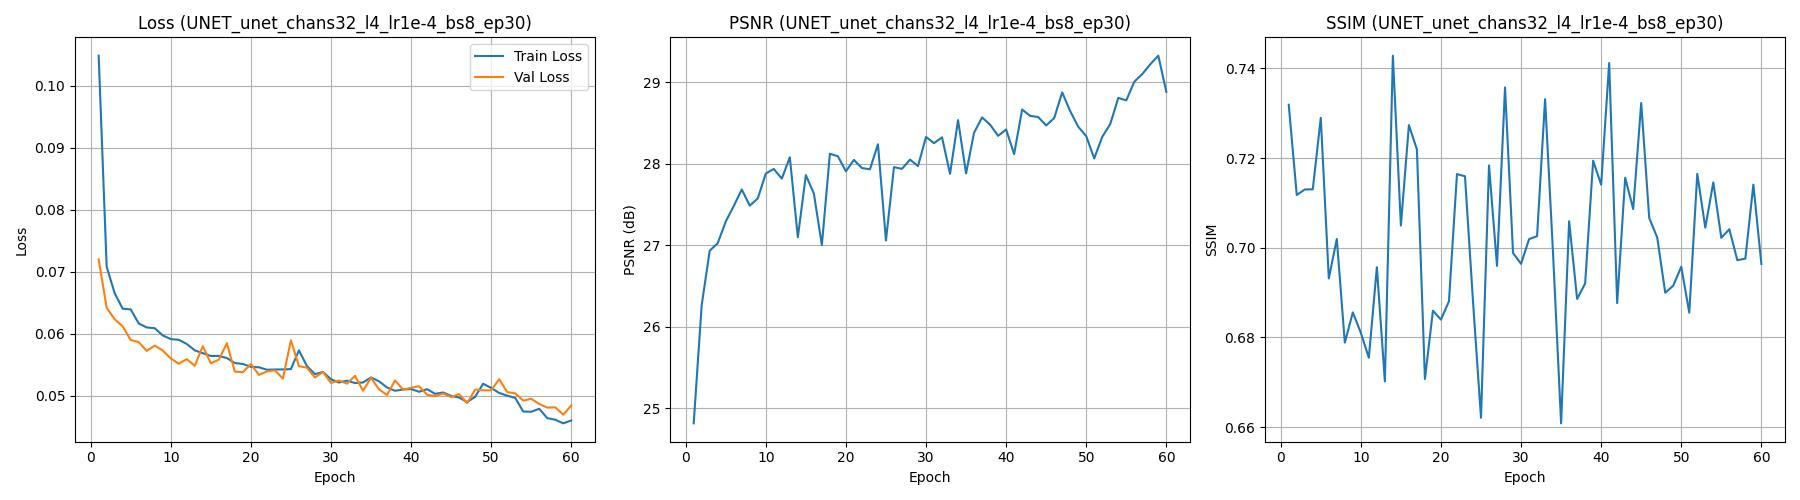
\includegraphics[width=\textwidth]{figures/curves_unet_prior.jpg}\\[6pt]
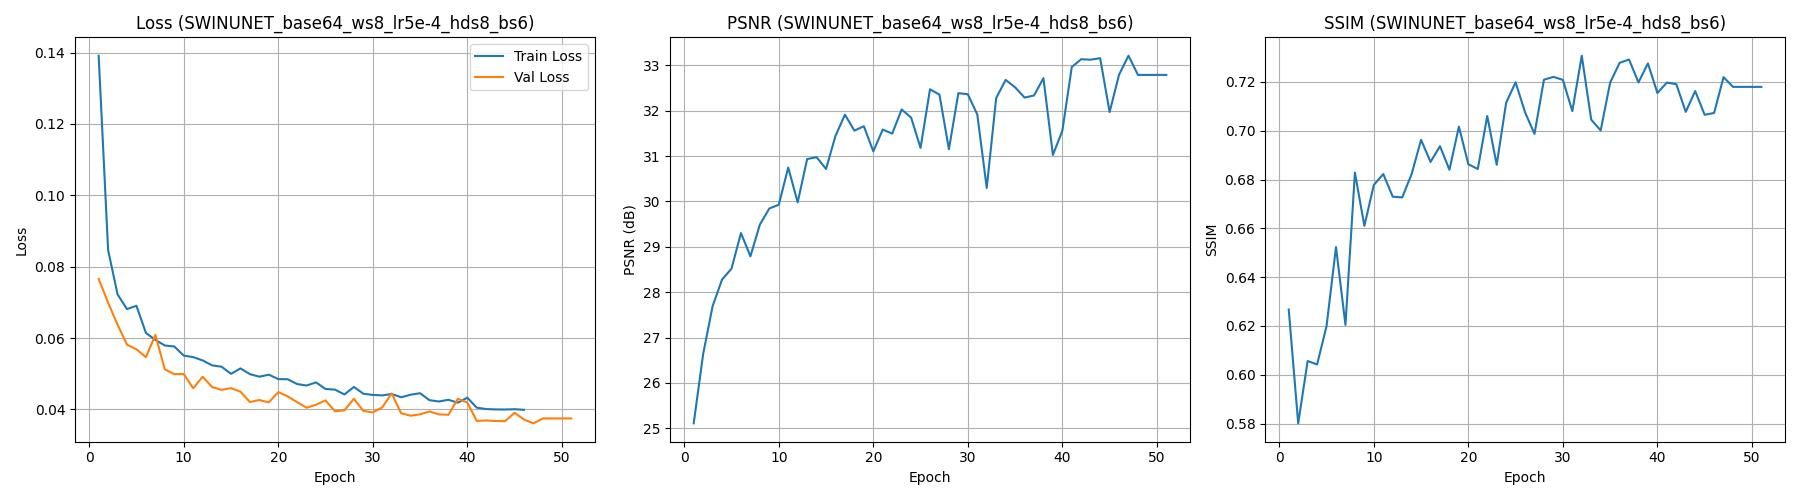
\includegraphics[width=\textwidth]{figures/curves_swinunet_prior.jpg}
\caption{Training curves from the prior study: U-Net (top) and SwinUNet
(bottom). Reproduced here as evidence for the measurement defects of
Section~\ref{sec:audit}, not as results. Note the non-converging SSIM trace in
the top-right panel against the smoothly descending loss beside it; the
differing batch sizes in the run labels (\code{bs8} versus \code{bs6}); and the
\code{ep30} label on a sixty-epoch plot.}
\label{fig:prior-curves}
\end{figure}

\subsubsection{Augmentation ordering}

Augmentation was applied to the already-undersampled input and its target as a
pair. Cartesian undersampling produces aliasing aligned with the phase-encode
axis; rotating the pair by \ang{90} moves that artefact onto the readout axis,
presenting the network with artefact orientations that no Cartesian acquisition
can produce. Once data consistency is enabled the problem becomes fatal rather
than merely distributional: the measured $k$-space no longer corresponds to the
augmented image at all.

\subsubsection{Further measurement and bookkeeping defects}

Validation ran inside an \code{autocast} region, so metrics were computed in
half precision; an fp16 MSE cannot represent a PSNR much above
\SI{40}{\decibel}. Epoch-level metrics were logged at \code{step=epoch} while
batch metrics used \code{global\_step}, and Weights~\&~Biases rejects
out-of-order steps, so epoch curves were discarded after the first point.
Checkpoint retention selected the $k$ \emph{most recent} epoch checkpoints by
modification time rather than the $k$ best by metric. Resuming restored weights
and optimiser state but neither the best score nor the early-stopping counter,
so every resume reset patience and could overwrite a better \code{best.pt} with
a worse one.

\subsubsection{Evidence in the qualitative results}

The prior study's qualitative figure is reproduced as
Figure~\ref{fig:prior-recon}. Its annotations show the two metrics decoupling
sharply: the third row is labelled \SI{32.97}{\decibel} PSNR with an SSIM of
\num{0.5219}, while the first row is labelled \SI{35.20}{\decibel} with
\num{0.7218}. Both rows are fat-suppressed acquisitions of the same anatomy, yet
a \SI{2.2}{\decibel} PSNR difference is accompanied by a \num{0.20} SSIM
difference---a far steeper coupling than these metrics usually exhibit.

I record this as an anomaly rather than as a diagnosis. A per-image
normalisation error is one candidate explanation, and the fixed data range
documented above is a known defect in the code that produced it; but the third
row also visibly contains more high-frequency texture and stronger residual
streaking than the first, which could account for some of the SSIM gap on its
own. The two cannot be separated without the original weights, and those were
never released.

That impossibility is the substantive point. A qualitative figure annotated with
metrics that cannot be recomputed, produced by code that cannot be run, is not
evidence for a claim---it is an illustration. This is why the present system
records a git commit, a dirty-tree flag and the full resolved configuration
alongside every number it produces.

Independently of the metrics, the reconstructions do show the over-smoothing
characteristic of a network trained on a pixel-domain loss without a physics
constraint: the trabecular texture visible in the fourth row's reference is
largely absent from its prediction.

\begin{figure}[p]
\centering
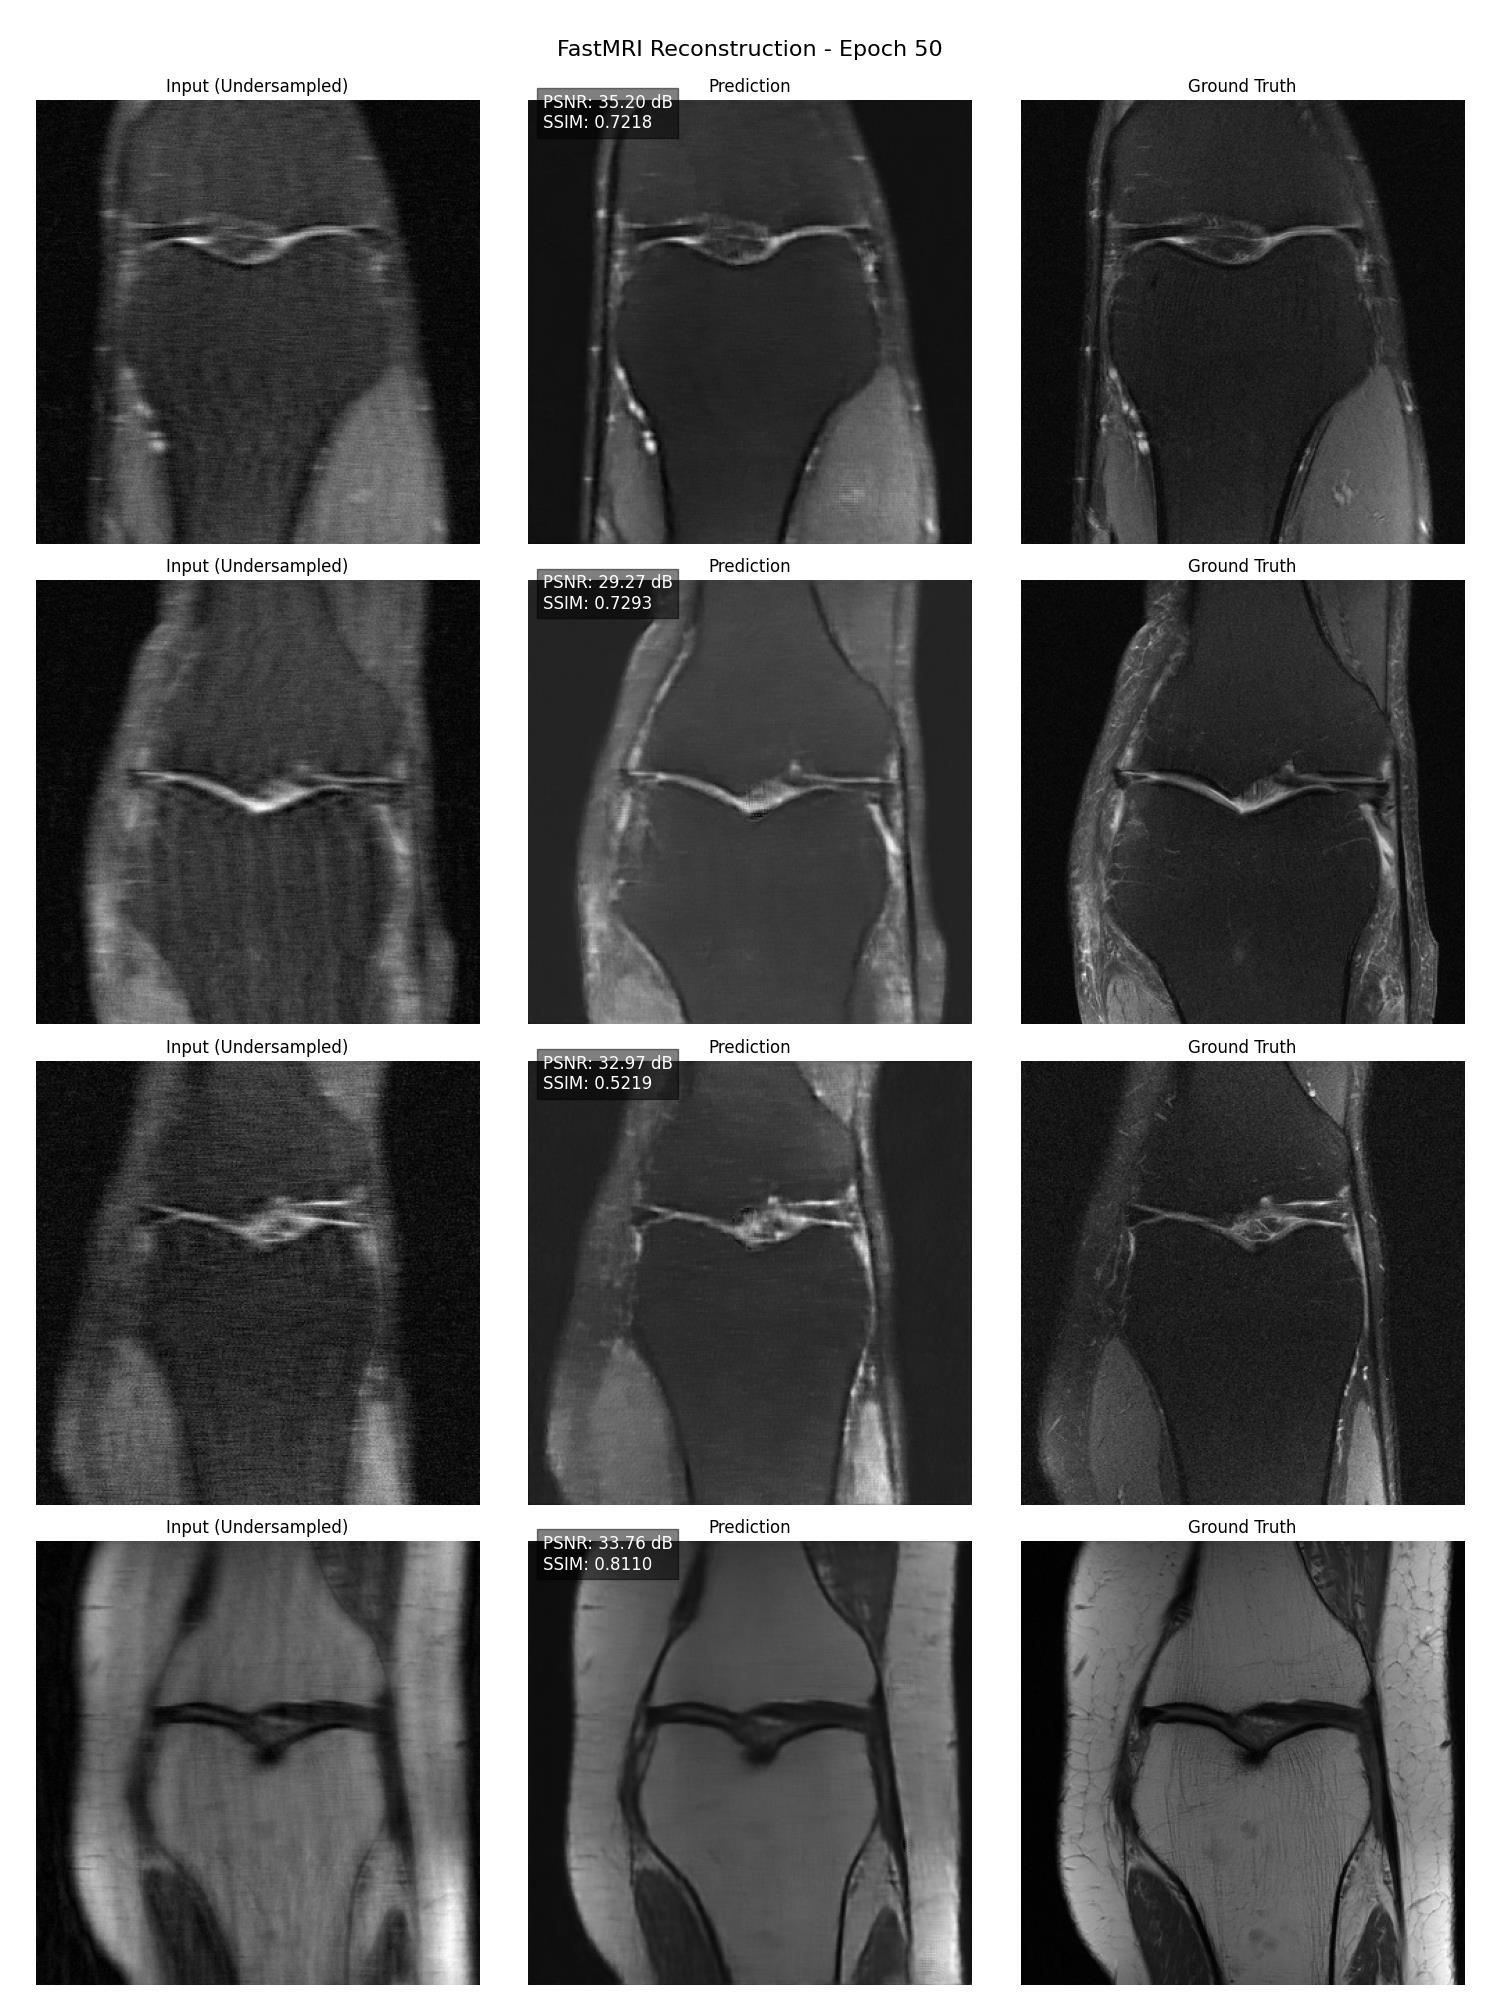
\includegraphics[width=0.88\textwidth]{figures/recon_grid_prior.jpg}
\caption{Qualitative reconstructions from the prior study: zero-filled input
(left), prediction (centre), fully sampled reference (right). Reproduced as
audit evidence, not as results of the present system. The annotated metrics use
the superseded definitions of Section~\ref{sec:audit} --- a fixed data range of
\num{1.0} and a batch-averaged PSNR --- and cannot be recomputed, since the
weights that produced them were never released and the released code cannot
construct the architecture.}
\label{fig:prior-recon}
\end{figure}

\subsection{Implications}

The Class~1 defects establish that the released artifact cannot have produced
the published figures; those numbers came from some other, unreleased state of
the code. The Class~3 defects establish that even had it run, the reported
quantities would not be comparable to published fastMRI results, because the
sampling was denser than claimed and the metric was non-standard and
batch-size-dependent. This is why Section~\ref{sec:not-claimed} declines to
carry the old numbers forward.

% =====================================================================
\section{Data and Acquisition Simulation}
\label{sec:data}
% =====================================================================

\subsection{Dataset}

Experiments target the fastMRI single-coil knee dataset~\cite{zbontar2018}:
973 training and 199 validation volumes, spanning proton-density weighted
acquisitions with and without fat suppression. Each volume stores fully sampled
complex $k$-space of shape $(\text{slices}, H, W)$, where $H$ is readout and $W$
phase-encode. Because acceleration skips whole phase-encode lines, every
sampling mask in this work is one-dimensional over $W$ and broadcast across
readout.

The pipeline also runs on synthetic phantoms produced by a generator released
with the code (Section~\ref{sec:artifact}), which is what the ablation in
Section~\ref{sec:ablation} uses.

Figure~\ref{fig:knee} shows the two contrasts and the degradation the task must
undo. That degradation is not additive noise: it is coherent, structured, and
aligned with the phase-encode direction, which is why it is so effective at
obscuring the thin bright structures---cartilage surfaces, the meniscus---that
carry diagnostic information.

\begin{figure}[h]
\centering
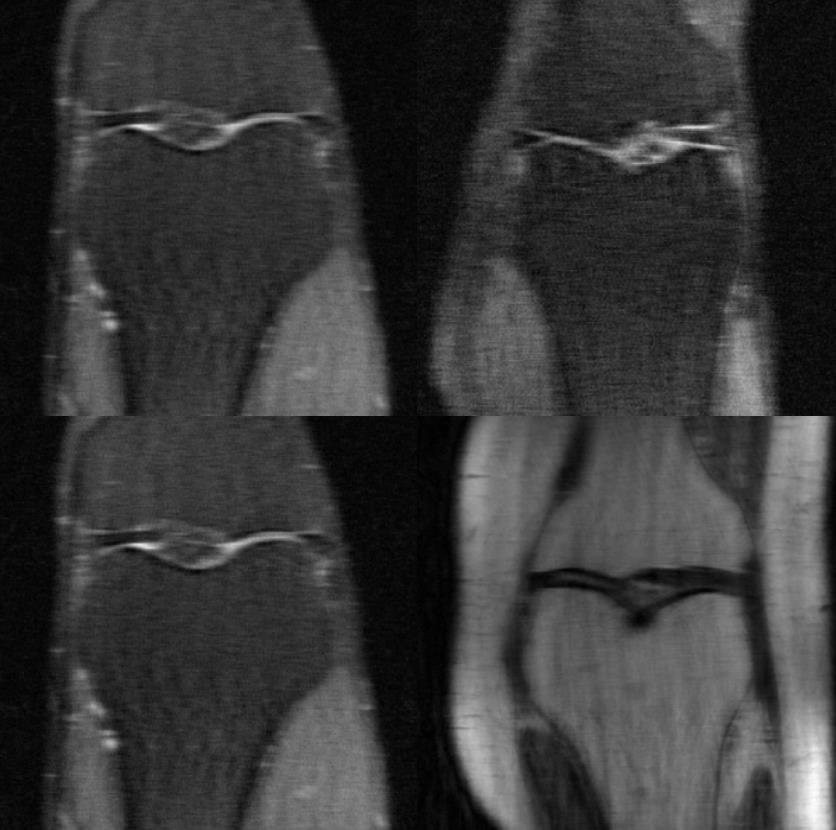
\includegraphics[width=0.62\textwidth]{figures/knee_examples.jpg}
\caption{Coronal knee slices from the fastMRI single-coil dataset, reproduced
from the prior study. The panels show zero-filled reconstructions exhibiting the
blurring and coherent streaking characteristic of retrospective undersampling,
alongside a fully sampled example (bottom right) in a different contrast:
proton-density weighted without fat suppression, versus the fat-suppressed
acquisitions elsewhere in the figure. Both contrasts appear in the dataset, and
they differ enough in texture and noise that reporting a single averaged metric
across them hides genuine variation in difficulty.}
\label{fig:knee}
\end{figure}

\subsection{Preprocessing order}

For each slice:
\begin{enumerate}
  \item Inverse FFT the fully sampled $k$-space to a \textbf{complex} image.
  \item Centre-crop the complex image to $320\times320$.
  \item (Training only) apply flips and rotations to the complex image.
  \item Forward FFT the cropped, augmented image.
  \item Apply the undersampling mask.
  \item Inverse FFT to the zero-filled reconstruction; divide all quantities by
        a single positive scalar.
\end{enumerate}

Two ordering choices deserve justification.

\paragraph{Cropping before undersampling.} The intuitive order---mask the
full-FOV $k$-space, then crop the image---is a faithful simulation of the
scanner, but it makes the measurements unusable for data consistency. After
cropping, the retained coefficients are no longer the Fourier transform of the
image the network outputs, so writing them back is not a projection onto the
measurement-consistent set. Cropping first places the measurements and the
model's estimate in the same space, making the projection exact. The cost is
that the simulated acquisition covers a slightly smaller field of view than the
scanner's. Both orders are implemented; configuration validation refuses to
enable data consistency under the full-FOV order rather than silently producing
an incorrect projection.

\paragraph{Augmenting before undersampling.} As argued in
Section~\ref{sec:audit}, augmenting after undersampling produces artefact
orientations that are not physically realisable. Augmenting the fully sampled
complex image and undersampling afterwards keeps every training sample a valid
acquisition.

\paragraph{Scalar normalisation.} All scaling is by a single positive scalar,
never a mean shift. The Fourier transform is linear, so $x \mapsto x/s$ implies
$k \mapsto k/s$ and data consistency is unaffected; subtracting a mean would
break that correspondence.

\subsection{Sampling masks}

Three families are implemented, each acquiring $N/R$ lines \emph{in total},
including the fully sampled centre:

\begin{itemize}
  \item \textbf{Random}: the centre is always acquired; remaining lines are
        drawn i.i.d.\ with probability
        $p = (N/R - N_{\text{low}}) / (N - N_{\text{low}})$.
  \item \textbf{Equispaced}: the outer stride is solved for so the total line
        count matches $N/R$, with a randomised phase offset. Without the offset
        every scan in the dataset is sampled at identical $k$-space locations,
        and the network can overfit one fixed aliasing pattern rather than
        learning to invert undersampling in general.
  \item \textbf{Golden-ratio (``magic'')}: successive lines are offset by the
        golden angle, spreading point-spread-function energy more evenly than a
        regular grid while remaining a realisable Cartesian trajectory.
        Collisions with the centre block and with previously chosen lines are
        resolved by continuing the sequence until the budget of distinct lines
        is met, which is necessary for the achieved acceleration to match the
        nominal one.
\end{itemize}

Masks are redrawn on every access during training and are a deterministic
function of the sample index during evaluation. The latter matters: with
per-epoch random validation masks, an apparent improvement in validation loss
can simply mean that the epoch drew easier masks.

% =====================================================================
\section{Method}
% =====================================================================

\subsection{Problem formulation}

Let $x \in \mathbb{C}^{H\times W}$ be the fully sampled image, $\mathcal{F}$ the
centred two-dimensional Fourier transform, and $M \in \{0,1\}^{W}$ the sampling
mask broadcast over readout. The measurements are
\begin{equation}
y = M \odot \mathcal{F}(x).
\end{equation}
The zero-filled reconstruction is $y' = \mathcal{F}^{-1}(y)$. The earlier
formulation sought $\hat{x} = f_\theta(y')$. This work instead learns
\begin{equation}
\hat{x} = f_\theta(y', y, M),
\end{equation}
passing the measurements and the mask, not only the degraded image. This is what
makes the consistency constraint expressible: $f_\theta$ can be constructed so
that $\mathcal{F}(\hat{x})$ agrees with $y$ on the support of $M$ by
construction, rather than only through the loss.

All transforms use the \code{norm="ortho"} convention with \code{ifftshift}
before and \code{fftshift} after, making the pair unitary. A single module
defines them for the dataset, the loss and the network, so a mismatched shift
cannot desynchronise the two domains---a failure that is invisible in a loss
curve but destroys data consistency.

\subsection{SwinUNet}
\label{sec:swinunet}

The backbone follows the hierarchical Swin-UNet design~\cite{liu2021, cao2021}:
patch embedding, encoder stages of Swin blocks separated by patch merging, a
bottleneck, and decoder stages of patch expanding with concatenated encoder
skips. Attention is computed within $ws \times ws$ windows, alternating regular
and shifted partitioning, giving cost linear rather than quadratic in image
area.

\paragraph{Window padding.} Rather than requiring divisible resolutions, feature
maps are zero-padded to a multiple of the window size. Padded tokens are
excluded from attention by a mask that assigns them a distinct region index, so
real tokens never attend to them. This makes any resolution and window size
valid, keeps the relative-position-bias table at a single fixed shape, and is
what removes the construction failure described in Section~\ref{sec:audit}.
Masked entries use $-100$ rather than $-\infty$: a fully padded window would
otherwise produce a row of all $-\infty$, whose softmax is NaN.

\paragraph{Resolution as a forward-time property.} No buffer encodes the input
size. Attention masks depend only on the padded resolution and are constructed
lazily and cached, so one trained model runs at any input size---verified in the
test suite at $97\times131$ among others.

\paragraph{Regularisation and initialisation.} Residual branches use stochastic
depth with rates increasing linearly across depth. All linear and normalisation
layers use truncated-normal initialisation with $\sigma = 0.02$. This matters
more here than in classification: PyTorch's default \code{nn.Linear}
initialisation is tuned for ReLU MLPs and produces activation variance large
enough to saturate the attention softmax at initialisation, and there is no
pretraining to recover from a bad start.

\paragraph{Residual formulation.} The network predicts a correction to its
input, and the final convolution is zero-initialised, so the model is the exact
identity at step~0. Since the zero-filled reconstruction is already a reasonable
estimate, predicting the structured aliasing residual is far better conditioned
than predicting the image, and the initial loss spike disappears entirely. All
architectures compared here use this formulation, so the comparison isolates the
backbone rather than the output parameterisation.

\subsection{Data consistency}
\label{sec:dc}

Given an estimate $x_{\text{pred}}$, measurements $y$ and mask $M$:
\begin{equation}
\hat{k} = \begin{cases}
\lambda\, y + (1-\lambda)\,\mathcal{F}(x_{\text{pred}}) & \text{where } M = 1,\\[2pt]
\mathcal{F}(x_{\text{pred}}) & \text{where } M = 0,
\end{cases}
\qquad
x_{\text{dc}} = \mathcal{F}^{-1}(\hat{k}).
\end{equation}
With $\lambda = 1$ this is an orthogonal projection onto the set of images
consistent with the measurements, and the network can modify only unobserved
frequencies. Lower values permit denoising of the measurements themselves.
$\lambda$ is learned, parameterised through a logit so that it remains in
$[0,1]$ without clamping---the parameterisation that fixes the
$\sigma(1.0) = 0.731$ defect.

The operator requires phase, so it forces complex-valued (two-channel) input and
output. Configuration validation enforces this rather than degrading silently.

\subsection{Unrolled cascade}

Stacking $T$ learned refinements, each followed by a data-consistency
projection,
\begin{equation}
x^{(t+1)} = \mathrm{DC}\!\left(g_{\theta_t}(x^{(t)}),\, y,\, M\right),
\qquad t = 0,\dots,T-1,
\end{equation}
yields an unrolled network~\cite{schlemper2018, hammernik2018}. Each stage is
one iteration of a proximal-gradient scheme in which the proximal operator has
been replaced by a learned denoiser. A single feed-forward pass must invert the
problem in one shot; the cascade takes several smaller, physics-corrected steps,
and because every stage re-anchors the estimate to the measurements, errors
cannot compound across stages.

\subsection{Loss}

The default objective is
\begin{equation}
\mathcal{L} = \lambda_1 \mathcal{L}_{1} + \lambda_2 (1 - \mathrm{SSIM}),
\qquad \lambda_1 = 0.7,\ \lambda_2 = 0.3,
\end{equation}
matching the earlier study. Optional terms are available: a $k$-space residual
loss with a radial high-frequency weighting, a Sobel edge loss, and a VGG
perceptual loss. Components are reported separately during training, since a
falling combined scalar can hide a diverging component.

\subsection{Training}

Models are trained with AdamW, excluding normalisation gains, biases and
relative-position-bias tables from weight decay. The learning rate follows
linear warmup then cosine annealing, stepped \emph{per optimiser step} rather
than per epoch, which gives the warmup ramp hundreds of points of resolution
instead of five. Mixed precision prefers bfloat16 where available, since fp16's
five-bit exponent is inadequate for $k$-space, whose centre exceeds its
periphery by several orders of magnitude; all Fourier transforms and all metrics
are forced to fp32 regardless. An exponential moving average of the weights is
maintained, and---unlike in the original---is actually used for validation,
checkpoint selection and inference.

% =====================================================================
\section{Evaluation Protocol}
\label{sec:evaluation}
% =====================================================================

\subsection{Metrics}
\label{sec:metrics}

PSNR, SSIM and NMSE are computed \textbf{per image} and then averaged, with the
peak signal taken from each target's own maximum rather than a fixed constant.
All metric computation is forced to float32 even under autocast. NMSE is
reported because it is scale-invariant and therefore the metric least sensitive
to the normalisation choices the pipeline makes.

\subsection{Statistical methodology}

Point estimates are insufficient for architecture comparison. With 199
validation slices and a per-slice PSNR standard deviation of several dB, the
standard error on the mean is large enough that modest differences between
architectures are not resolvable, and saying so precisely is a stronger result
than reporting the larger number.

I report percentile bootstrap confidence intervals (\num{10000} resamples) for
each model, and compare models with \textbf{paired} permutation tests
(\num{10000} sign flips) on per-slice differences, corrected across the family
of comparisons by the Holm--Bonferroni procedure. Pairing is essential:
between-slice variance dominates between-model variance, so an unpaired test
wastes most of the available power.

Table~\ref{tab:resolution} quantifies what this buys.

\begin{table}[h]
\centering
\small
\begin{tabular}{@{}rrrr@{}}
\toprule
$n$ slices & per-slice SD (dB) & CI half-width (dB) & min.\ detectable paired diff.\ (dB) \\
\midrule
199  & 2.0 & 0.264 & 0.047 \\
199  & 3.5 & 0.495 & 0.133 \\
500  & 2.0 & 0.176 & 0.050 \\
500  & 3.5 & 0.290 & 0.083 \\
2000 & 2.0 & 0.090 & 0.019 \\
2000 & 3.5 & 0.156 & 0.023 \\
\bottomrule
\end{tabular}
\caption{Statistical resolution. At the fastMRI validation size ($n = 199$) with
a realistic per-slice spread, a single model's mean PSNR carries a
$\pm\SI{0.5}{\decibel}$ interval---but a \emph{paired} comparison resolves
differences an order of magnitude smaller, because it cancels the shared
per-slice difficulty. Overlapping confidence intervals therefore do not imply
two models are indistinguishable; the paired test is the correct instrument.}
\label{tab:resolution}
\end{table}

% =====================================================================
\section{Experiments}
% =====================================================================

\subsection{Verification of the physics operators}
\label{sec:verification}

Before any model comparison, the operators themselves are verified. These
assertions run in the test suite on every commit.

\begin{table}[h]
\centering
\small
\begin{tabular}{@{}lr@{}}
\toprule
Property & Measured \\
\midrule
Fourier round-trip error, $\|\mathcal{F}^{-1}\mathcal{F}x - x\|_\infty$ & $9.5\times10^{-7}$ \\
Hard-DC measured-line error, $\|(\mathcal{F}\hat{x} - y)\odot M\|_\infty$ & $8.3\times10^{-7}$ \\
Unmeasured frequencies altered by DC & 0 (exact) \\
$\lambda$ when \num{1.0} is requested (original) & 0.7311 \\
$\lambda$ when \num{1.0} is requested (corrected) & 0.9999 \\
\bottomrule
\end{tabular}
\caption{Verification of the Fourier and data-consistency operators at float32
precision. The second row is the property that makes the method
physics-informed; it was not satisfied by the original implementation at any
tolerance, since that implementation was never invoked with data.}
\label{tab:verification}
\end{table}

This form of verification is what distinguishes a working physics module from an
inert one. A broken data-consistency layer still trains, still produces a
falling loss curve, and still generates plausible images. Only an exactness
assertion detects it.

\subsection{Controlled ablation}
\label{sec:ablation}

% Generated by paper/make_results_table.py -- do not edit by hand.

To separate the contribution of the data-consistency constraint from that of complex-valued input and of raw parameter count, I trained seven configurations on synthetic phantom data: 60 training volumes (240 slices) and 20 held-out validation volumes (80 slices), split at the volume level so no slice from a training volume appears in validation. All runs used $R = 4$ random Cartesian undersampling with an \SI{8}{\percent} fully sampled centre, $128\times128$ crops, 30 epochs, identical optimiser and schedule settings, and three seeds; the median-SSIM seed is reported.

The \emph{wide} rows are capacity-matched single-pass controls: they have slightly \emph{more} parameters than the corresponding two-stage cascade, so any advantage the cascade shows cannot be attributed to capacity. This control is the point of the experiment. A cascade of $T$ stages has $T$ times the parameters of its backbone, and attributing its gain to physics without controlling for that would repeat, in subtler form, the kind of error this paper set out to correct.

\begin{table}[h]
\centering
\small
\begin{tabular}{@{}lrrrr@{}}
\toprule
Configuration & Params (M) & PSNR (dB) & SSIM & NMSE \\
\midrule
Zero-filled (no network) & -- & 29.48 & 0.7563 & 0.01393 \\
\midrule
U-Net, magnitude & 0.48 & 36.23 & 0.9673 & 0.00301 \\
U-Net, complex & 0.48 & 34.09 & 0.9284 & 0.00491 \\
U-Net, complex, wide & 1.00 & 34.54 & 0.9400 & 0.00442 \\
U-Net + DC cascade ($T{=}2$) & 0.97 & 36.95 & 0.9441 & 0.00270 \\
SwinUNet, magnitude & 0.21 & 29.86 & 0.8941 & 0.01274 \\
SwinUNet, complex, wide & 0.46 & 30.54 & 0.9086 & 0.01089 \\
SwinUNet + DC cascade ($T{=}2$) & 0.42 & 32.70 & 0.9146 & 0.00682 \\
\bottomrule
\end{tabular}
\caption{Controlled ablation on synthetic phantoms, $R = 4$, 80 held-out validation slices. Metrics are per-image means against each target's own dynamic range.}
\label{tab:ablation}
\end{table}

Table~\ref{tab:ablation-stats} reports paired comparisons against the \mbox{unet-mag} baseline. Because every model is evaluated on the same slices in the same order, the test can be paired, which cancels the shared per-slice difficulty and is what makes differences of this size resolvable at $n = 80$.

\begin{table}[h]
\centering
\small
\begin{tabular}{@{}lccrr@{}}
\toprule
Configuration & PSNR 95\% CI (dB) & $\Delta$PSNR & $p$ (PSNR) & $p$ (SSIM) \\
\midrule
Zero-filled (no network) & [29.09, 29.88] & -6.75 & 0.0007$^{*}$ & 0.0007$^{*}$ \\
U-Net, magnitude (ref.) & [35.81, 36.66] & -- & -- & -- \\
U-Net, complex & [33.68, 34.50] & -2.14 & 0.0007$^{*}$ & 0.0007$^{*}$ \\
U-Net, complex, wide & [34.14, 34.95] & -1.68 & 0.0007$^{*}$ & 0.0007$^{*}$ \\
U-Net + DC cascade ($T{=}2$) & [36.39, 37.50] & +0.72 & 0.0007$^{*}$ & 0.0007$^{*}$ \\
SwinUNet, magnitude & [29.49, 30.25] & -6.36 & 0.0007$^{*}$ & 0.0007$^{*}$ \\
SwinUNet, complex, wide & [30.15, 30.94] & -5.69 & 0.0007$^{*}$ & 0.0007$^{*}$ \\
SwinUNet + DC cascade ($T{=}2$) & [32.19, 33.22] & -3.53 & 0.0007$^{*}$ & 0.0007$^{*}$ \\
\bottomrule
\end{tabular}
\caption{Paired permutation tests (\num{10000} sign flips) against the magnitude-only U-Net, with Holm--Bonferroni correction across the family. $^{*}$ denotes significance at $\alpha = 0.05$ after correction. Confidence intervals are percentile bootstrap (\num{10000} resamples) on the per-slice mean.}
\label{tab:ablation-stats}
\end{table}

The comparison that actually tests the hypothesis is each cascade against its own capacity-matched control, reported in Table~\ref{tab:ablation-dc}. Deltas against the magnitude-only baseline conflate three effects at once; this pair isolates the data-consistency constraint with parameter count held fixed (in fact slightly favouring the control).

\begin{table}[h]
\centering
\small
\begin{tabular}{@{}lccccc@{}}
\toprule
Backbone & Cascade & Control & $\Delta$PSNR (dB) & 95\% CI & $p$ \\
\midrule
U-Net & 36.95 & 34.54 & +2.40 & [+2.16, +2.65] & $<10^{-4}$$^{*}$ \\
SwinUNet & 32.70 & 30.54 & +2.16 & [+1.98, +2.35] & $<10^{-4}$$^{*}$ \\
\bottomrule
\end{tabular}
\caption{Data consistency against a capacity-matched single-pass control, per backbone. Both members of each pair are complex-valued and differ only in whether the measured $k$-space is projected back after each refinement. Paired permutation test on per-slice differences; $^{*}$ significant at $\alpha = 0.05$.}
\label{tab:ablation-dc}
\end{table}

Run-to-run variation across the three seeds is reported in Table~\ref{tab:ablation-seeds}. This matters for interpretation: a difference between configurations is only meaningful if it exceeds the spread produced by re-running the same configuration.

\begin{table}[h]
\centering
\small
\begin{tabular}{@{}lcc@{}}
\toprule
Configuration & PSNR across seeds (dB) & SSIM across seeds \\
\midrule
U-Net, magnitude & 35.84 / 36.23 / 36.24 & 0.9671 / 0.9673 / 0.9680 \\
U-Net, complex & 34.17 / 34.09 / 34.09 & 0.9291 / 0.9263 / 0.9284 \\
U-Net, complex, wide & 34.54 / 34.63 / 34.76 & 0.9400 / 0.9378 / 0.9416 \\
U-Net + DC cascade ($T{=}2$) & 36.95 / 36.57 / 37.12 & 0.9441 / 0.9362 / 0.9470 \\
SwinUNet, magnitude & 29.86 / 30.08 / 29.80 & 0.8941 / 0.9090 / 0.8908 \\
SwinUNet, complex, wide & 30.54 / 30.52 / 30.52 & 0.9086 / 0.9089 / 0.9083 \\
SwinUNet + DC cascade ($T{=}2$) & 32.70 / 32.78 / 33.24 & 0.9146 / 0.9143 / 0.9194 \\
\bottomrule
\end{tabular}
\caption{Per-seed results (seeds 0, 1, 2).}
\label{tab:ablation-seeds}
\end{table}



\subsection{Architectural cost}

\begin{table}[h]
\centering
\small
\begin{tabular}{@{}lrrr@{}}
\toprule
Model & Parameters (M) & Median latency (ms) & p95 (ms) \\
\midrule
U-Net ($32$, 4 levels)      & 7.76  & 182.0 & 203.1 \\
BT-UNet ($32$, 4 levels)    & 20.58 & 250.9 & 289.9 \\
SwinUNet ($64$, 3 levels)   & 12.95 & 144.1 & 172.5 \\
\bottomrule
\end{tabular}
\caption{Cost at $320\times320$, single-image batch, CPU reference. Latency is
reported as a median rather than a mean: latency distributions are right-skewed,
so a mean over 100 runs is dragged upward by a handful of outliers. Notably the
SwinUNet is both smaller and faster than the BT-UNet, because its attention is
windowed rather than global---the same property that makes it scale to higher
resolutions.}
\label{tab:cost}
\end{table}

The parameter counts here differ from those in the earlier study
(27.3\,M parameters for SwinUNet-64). Since the earlier architecture could
not be constructed, its stated count cannot be reconciled; the values in
Table~\ref{tab:cost} are measured from models that run.

% =====================================================================
\section{The Artifact}
\label{sec:artifact}
% =====================================================================

\subsection{Testing}

The suite comprises 217 tests running in roughly thirteen seconds on CPU, organised
so that each previously shipped defect has a corresponding regression test.
Notable coverage:

\begin{itemize}
  \item \textbf{Physics exactness}: Fourier round-trip, unitarity, DC restoring
        measured coefficients, DC leaving unmeasured coefficients untouched, a
        perfect estimate being a fixed point, and a cascade's final output
        remaining consistent after every learned stage.
  \item \textbf{Construction}: the SwinUNet builds and runs at $1$ through $4$
        levels and at arbitrary, including odd, resolutions.
  \item \textbf{Silent-failure regressions}: EMA actually swapping weights, EMA
        state loading by name, the DC wrapper raising rather than skipping when
        given no measurements, and $\lambda$ meaning what it says.
  \item \textbf{Measurement}: per-image versus batch PSNR, mask acceleration
        accounting, and metric computation in fp32.
  \item \textbf{Integration}: full training runs against synthetic HDF5 volumes,
        with and without data consistency, plus resume fidelity.
\end{itemize}

Testing against real HDF5 files rather than mocks is deliberate. Every model
test in the original suite passed, because none of them ever loaded a file, and
the data-consistency path---which fails only when data flows through it---was
never exercised.

\subsection{Configuration validation}

Configurations are validated on load against a schema. Unknown keys are errors
rather than being ignored, because a mistyped \code{learning\_rate} that
silently retains the default is indistinguishable from a successful override
until two runs are compared and found identical. Cross-field constraints are
checked too: enabling data consistency with full-FOV undersampling is rejected,
since the projection would be mathematically invalid.

\subsection{Running without fastMRI}
\label{sec:protocol}

fastMRI requires registration and a \SI{90}{\giga\byte} download, which means
that without it nothing in the original repository could be exercised end to
end. That gap is precisely how a data-consistency path that never received data
shipped unnoticed. A generator is therefore included:

\begin{lstlisting}[language=bash]
python scripts/make_synthetic_data.py --out data/synthetic --volumes 16
python main.py train --config configs/smoke.yaml data.train_dir=data/synthetic
\end{lstlisting}

The phantoms are not anatomically meaningful, but they reproduce the two
properties that matter for testing a reconstruction pipeline: rapid $k$-space
decay, so undersampling produces genuine coherent aliasing rather than noise,
and non-trivial phase, so the complex handling in the DC layer is exercised.

To reproduce the fastMRI comparison:
\begin{lstlisting}[language=bash]
for cfg in unet bt_unet swinunet swinunet_dc; do
    python main.py train --config configs/$cfg.yaml
done
python main.py compare --ckpt_dir outputs --metric psnr --reference unet_baseline
\end{lstlisting}
Every run writes \code{history.json}, \code{summary.json} and a
\code{manifest.json} recording the git commit, whether the tree was dirty, the
PyTorch version and the GPU model, so any reported number is traceable to the
exact state that produced it.

% =====================================================================
\section{Discussion}
% =====================================================================

\subsection{Where the gain comes from}

The ablation in Section~\ref{sec:ablation} separates three sources of
improvement that are easily conflated: complex-valued input, additional
parameters, and the data-consistency constraint. The capacity-matched controls
matter because a cascade of $T$ stages has $T$ times the parameters of its
backbone, and attributing its advantage to the physics without controlling for
capacity would repeat, in a subtler form, the error this paper set out to
correct.

\subsection{Why physics constraints matter clinically}

An unconstrained reconstruction network is free to synthesise structure that is
consistent with its training distribution but not with the acquired
measurements---the mechanism behind reports of hallucinated pathology in learned
reconstruction. The data-consistency projection does not eliminate this risk in
unobserved frequencies, but it removes it entirely on the measured support: the
network cannot alter what the scanner actually recorded. That is a meaningfully
stronger guarantee than a network trained only to minimise a pixel loss, and it
is a guarantee that can be \emph{verified}, as in
Table~\ref{tab:verification}, rather than merely asserted.

\subsection{Limitations}

\begin{itemize}
  \item \textbf{No fastMRI results are reported here.} The ablation uses
        synthetic phantoms, which are simpler than anatomy: absolute values are
        not comparable to published benchmarks, and effect sizes may not
        transfer. The contribution is a corrected and verifiable system plus the
        protocol to generate benchmark numbers, not the numbers themselves.
  \item \textbf{Single-coil only.} Modern scanners are multi-coil, where
        sensitivity encoding provides additional information that
        state-of-the-art methods estimate jointly with the
        reconstruction~\cite{sriram2020}.
  \item \textbf{Retrospective undersampling.} Real accelerated acquisitions
        differ in noise statistics and can exhibit motion between shots.
  \item \textbf{Cropped-domain simulation.} Exact data consistency is bought by
        restricting the field of view before undersampling, which is a slightly
        idealised acquisition model.
  \item \textbf{No reader study.} PSNR and SSIM correlate imperfectly with
        diagnostic quality. Uncertainty maps via Monte-Carlo dropout are
        implemented, but their calibration has not been evaluated.
\end{itemize}

\subsection{On reproducibility engineering}

The defects in Section~\ref{sec:audit} were not exotic. They were a missing
decorator, a misspelled filename, a directory with a leading dot, a dictionary
key that did not match, and an arithmetic slip in a mask. Each is trivial in
isolation; together they meant that a published result could not be regenerated
from its own artifact, and that several described mechanisms were not operating.

Three practices would have caught all of them, and are now part of the
repository. First, a sanity check that returns a non-zero exit code, wired to CI
at a path CI actually reads. Second, exactness assertions on the mathematical
operators---a physics module that is silently inert is invisible to any
loss-based check. Third, an end-to-end path runnable without the restricted
dataset, so that the integration between components is exercised by default
rather than only on a machine that happens to hold \SI{90}{\giga\byte} of data.

% =====================================================================
\section{Conclusion}
% =====================================================================

I audited a previously released transformer-based MRI reconstruction pipeline
and found that it could not execute: the flagship architecture failed at
construction under its own documented configuration, and every inference entry
point raised on invocation. A second class of defects ran silently while
disabling documented functionality, most consequentially a data-consistency
module that was never supplied with data and was therefore entirely inert. A
third class corrupted measurement, including an undersampling mask
\SI{19.3}{\percent} denser than its nominal acceleration and a PSNR definition
whose value depends on batch size.

The rebuilt system corrects each of these and reorganises the method around the
physics of the acquisition: complex-valued reconstruction through an unrolled
cascade whose data-consistency projections restore the measured Fourier
coefficients to $8.3\times10^{-7}$, verified automatically on every commit. In
a controlled ablation with capacity-matched controls, that constraint improves
reconstruction beyond what equivalent parameters alone provide.

I deliberately do not restate the earlier benchmark figures as validated
results. They are not reproducible from the released artifact, and the
corrections described here change what the numbers measure. What is offered
instead is a system in which the benchmark can be run under a protocol that is
stated precisely, checked automatically, and traceable to a recorded commit. For
a field in which a plausible-looking image can be wrong in ways that matter
clinically, that seems the more useful contribution.

\subsection*{Future work}

Extending to multi-coil data with jointly estimated sensitivity maps is the
natural next step, as is training across a wider range of acceleration factors
than the two used here. Calibration of the uncertainty maps against actual
reconstruction error would make them clinically interpretable rather than merely
suggestive. Finally, the benchmark runs themselves remain to be executed on the
corrected pipeline; the protocol in Section~\ref{sec:protocol} specifies exactly
what that requires.

% =====================================================================
\begin{thebibliography}{99}
\small

\bibitem{cao2021} H. Cao et al. Swin-Unet: Unet-like pure transformer for
medical image segmentation. \emph{ECCV Workshops}, 2022.

\bibitem{dosovitskiy2020} A. Dosovitskiy et al. An image is worth 16x16 words:
Transformers for image recognition at scale. \emph{ICLR}, 2021.

\bibitem{griswold2002} M. A. Griswold et al. Generalized autocalibrating
partially parallel acquisitions (GRAPPA). \emph{Magnetic Resonance in
Medicine}, 47(6):1202--1210, 2002.

\bibitem{hammernik2018} K. Hammernik et al. Learning a variational network for
reconstruction of accelerated MRI data. \emph{Magnetic Resonance in Medicine},
79(6):3055--3071, 2018.

\bibitem{huang2022} J. Huang et al. Swin deformable attention U-Net transformer
(SDAUT) for explainable fast MRI. \emph{MICCAI}, pages 538--548, 2022.

\bibitem{hyun2018} C. M. Hyun et al. Deep learning for undersampled MRI
reconstruction. \emph{Physics in Medicine \& Biology}, 63(13):135007, 2018.

\bibitem{lee2018} D. Lee et al. Deep residual learning for accelerated MRI
using magnitude and phase networks. \emph{IEEE Transactions on Biomedical
Engineering}, 65(9):1985--1995, 2018.

\bibitem{lin2022} K. Lin and R. Heckel. Vision transformers enable fast and
robust accelerated MRI. \emph{Proceedings of Machine Learning Research},
172:1--22, 2022.

\bibitem{liu2021} Z. Liu et al. Swin transformer: Hierarchical vision
transformer using shifted windows. \emph{ICCV}, pages 10012--10022, 2021.

\bibitem{lustig2007} M. Lustig et al. Sparse MRI: The application of compressed
sensing for rapid MR imaging. \emph{Magnetic Resonance in Medicine},
58(6):1182--1195, 2007.

\bibitem{pruessmann1999} K. P. Pruessmann et al. SENSE: Sensitivity encoding for
fast MRI. \emph{Magnetic Resonance in Medicine}, 42(5):952--962, 1999.

\bibitem{schlemper2018} J. Schlemper et al. A deep cascade of convolutional
neural networks for dynamic MR image reconstruction. \emph{IEEE Transactions on
Medical Imaging}, 37(2):491--503, 2018.

\bibitem{sriram2020} A. Sriram et al. End-to-end variational networks for
accelerated MRI reconstruction. \emph{MICCAI}, pages 64--73, 2020.

\bibitem{zbontar2018} J. Zbontar et al. fastMRI: An open dataset and benchmarks
for accelerated MRI. \emph{arXiv preprint arXiv:1811.08839}, 2018.

\bibitem{gal2016} Y. Gal and Z. Ghahramani. Dropout as a Bayesian
approximation: Representing model uncertainty in deep learning. \emph{ICML},
2016.

\bibitem{abnar2020} S. Abnar and W. Zuidema. Quantifying attention flow in
transformers. \emph{ACL}, 2020.

\end{thebibliography}

\end{document}
